\documentclass[11pt,a4paper]{article}
\usepackage[utf8]{inputenc}
\usepackage[T1]{fontenc}
\usepackage{tgpagella}
\usepackage[spanish]{babel}
\usepackage{geometry}
\usepackage{booktabs}
\usepackage{xcolor}
\usepackage{titlesec}
\usepackage{fancyhdr}
\usepackage[parfill]{parskip}
\usepackage[expansion=false]{microtype}
\usepackage{hyperref}
\usepackage{setspace}
\usepackage{needspace}
\usepackage{graphicx}
\widowpenalty=10000
\clubpenalty=10000
\displaywidowpenalty=10000

\geometry{top=3.0cm,bottom=3.0cm,left=3.5cm,right=3.5cm}
\setlength{\parskip}{0.65em}
\setlength{\parindent}{0em}

\definecolor{azulai}{RGB}{30,80,140}
\definecolor{doradoai}{RGB}{140,90,0}
\definecolor{grisai}{RGB}{70,70,70}

\titleformat{\section}{\Large\bfseries\color{azulai}}{}{0em}{}[{\color{azulai}\titlerule[0.5pt]}]
\titlespacing*{\section}{0pt}{1.8em}{0.8em}
\titleformat{\subsection}{\large\bfseries\color{doradoai}}{}{0em}{}
\titlespacing*{\subsection}{0pt}{1.4em}{0.5em}
\titleformat{\subsubsection}{\normalsize\bfseries\color{grisai}}{}{0em}{}
\titlespacing*{\subsubsection}{0pt}{1.0em}{0.3em}

\pagestyle{fancy}\fancyhf{}
\rhead{\textcolor{grisai}{\small Raquel Pain — Arquitectura Interna}}
\lhead{\textcolor{grisai}{\small Júpiter · Saturno}}
\cfoot{\textcolor{grisai}{\small\thepage}}
\renewcommand{\headrulewidth}{0.3pt}

\hypersetup{colorlinks=true,linkcolor=azulai,urlcolor=azulai}
\setstretch{1.45}
\tolerance=1500
\emergencystretch=4em

\begin{document}

% ── Portada ──────────────────────────────────────────────────────────────────

\begin{titlepage}
\centering

\vspace*{2cm}

{\Huge\bfseries\color{azulai} Júpiter · Saturno}\\[0.4cm]

{\large\color{grisai} Arquitectura Interna}\\[0.25cm]

{\small\itshape\color{grisai}
Crecimiento, estructura y organización interna
}\\[1.8cm]

{\huge\color{doradoai} Raquel Pain}\\[1.2cm]

{\Large 07/05/1985 \quad 18:20}\\[0.25cm]

{\Large Pamplona, España}\\[0.25cm]

{\normalsize
Lat: 42.8157° \quad
Lon: -1.6522° \quad
UTC+02:00
}\\[0.4cm]

{\normalsize
Ascendente: Libra 14°36'
\quad
MC: Cáncer 17°21'
}\\[1.6cm]

\begin{tabular}{ll}
\textbf{Júpiter:} & Acuario — Casa 4 15°44' \\
\textbf{Saturno:} & Escorpio — Casa 2 25°26' (Retrógrado) \\
\end{tabular}

\vfill

{\small\color{grisai}
Generado el 20/05/2026
}

\end{titlepage}

	ableofcontents
space{0.8cm}

% ── Datos de referencia ──────────────────────────────────────────────────────

\section{Datos de referencia}

\begin{center}
\begin{tabular}{llll}
\toprule
\textbf{Punto} & \textbf{Signo} & \textbf{Casa} & \textbf{Posición} \\
\midrule

Júpiter &
Acuario &
Casa 4 &
15°44' \\

Saturno (Retrógrado) &
Escorpio &
Casa 2 &
25°26' \\

Sol &
Tauro &
Casa 8 &
17°02' \\

Luna &
Sagitario &
Casa 3 &
26°31' \\

Mercurio &
Aries &
Casa 7 &
21°12' \\

Venus &
Aries &
Casa 6 &
8°52' \\

Marte &
Géminis &
Casa 8 &
7°49' \\

Urano &
Sagitario &
Casa 3 &
17°09' \\

Ascendente &
Libra &
--- &
14°36' \\

Medio Cielo &
Cáncer &
--- &
17°21' \\

\bottomrule
\end{tabular}
\end{center}

\vspace{0.8cm}

\subsection*{Aspectos entre funciones}

\begin{center}
\begin{tabular}{lllll}
  \toprule
  \textbf{Planeta 1} & \textbf{Asp.} & \textbf{Planeta 2} & \textbf{Tipo} & \textbf{Orbe} \\
  \midrule
  Júpiter & cua & Sol & Cuadratura & 1.3° \\
  Júpiter & sex & Urano & Sextil & 1.4° \\
  Júpiter & sex & Mercurio & Sextil & 5.5° \\
  Júpiter & tri & Quirón & Trígono & 7.2° \\
  Júpiter & tri & Marte & Trígono & 7.9° \\
  Saturno & opo & Sol & Oposición & 8.4° \\
  \bottomrule
\end{tabular}
\end{center}

\vspace{1cm}

\begin{center}
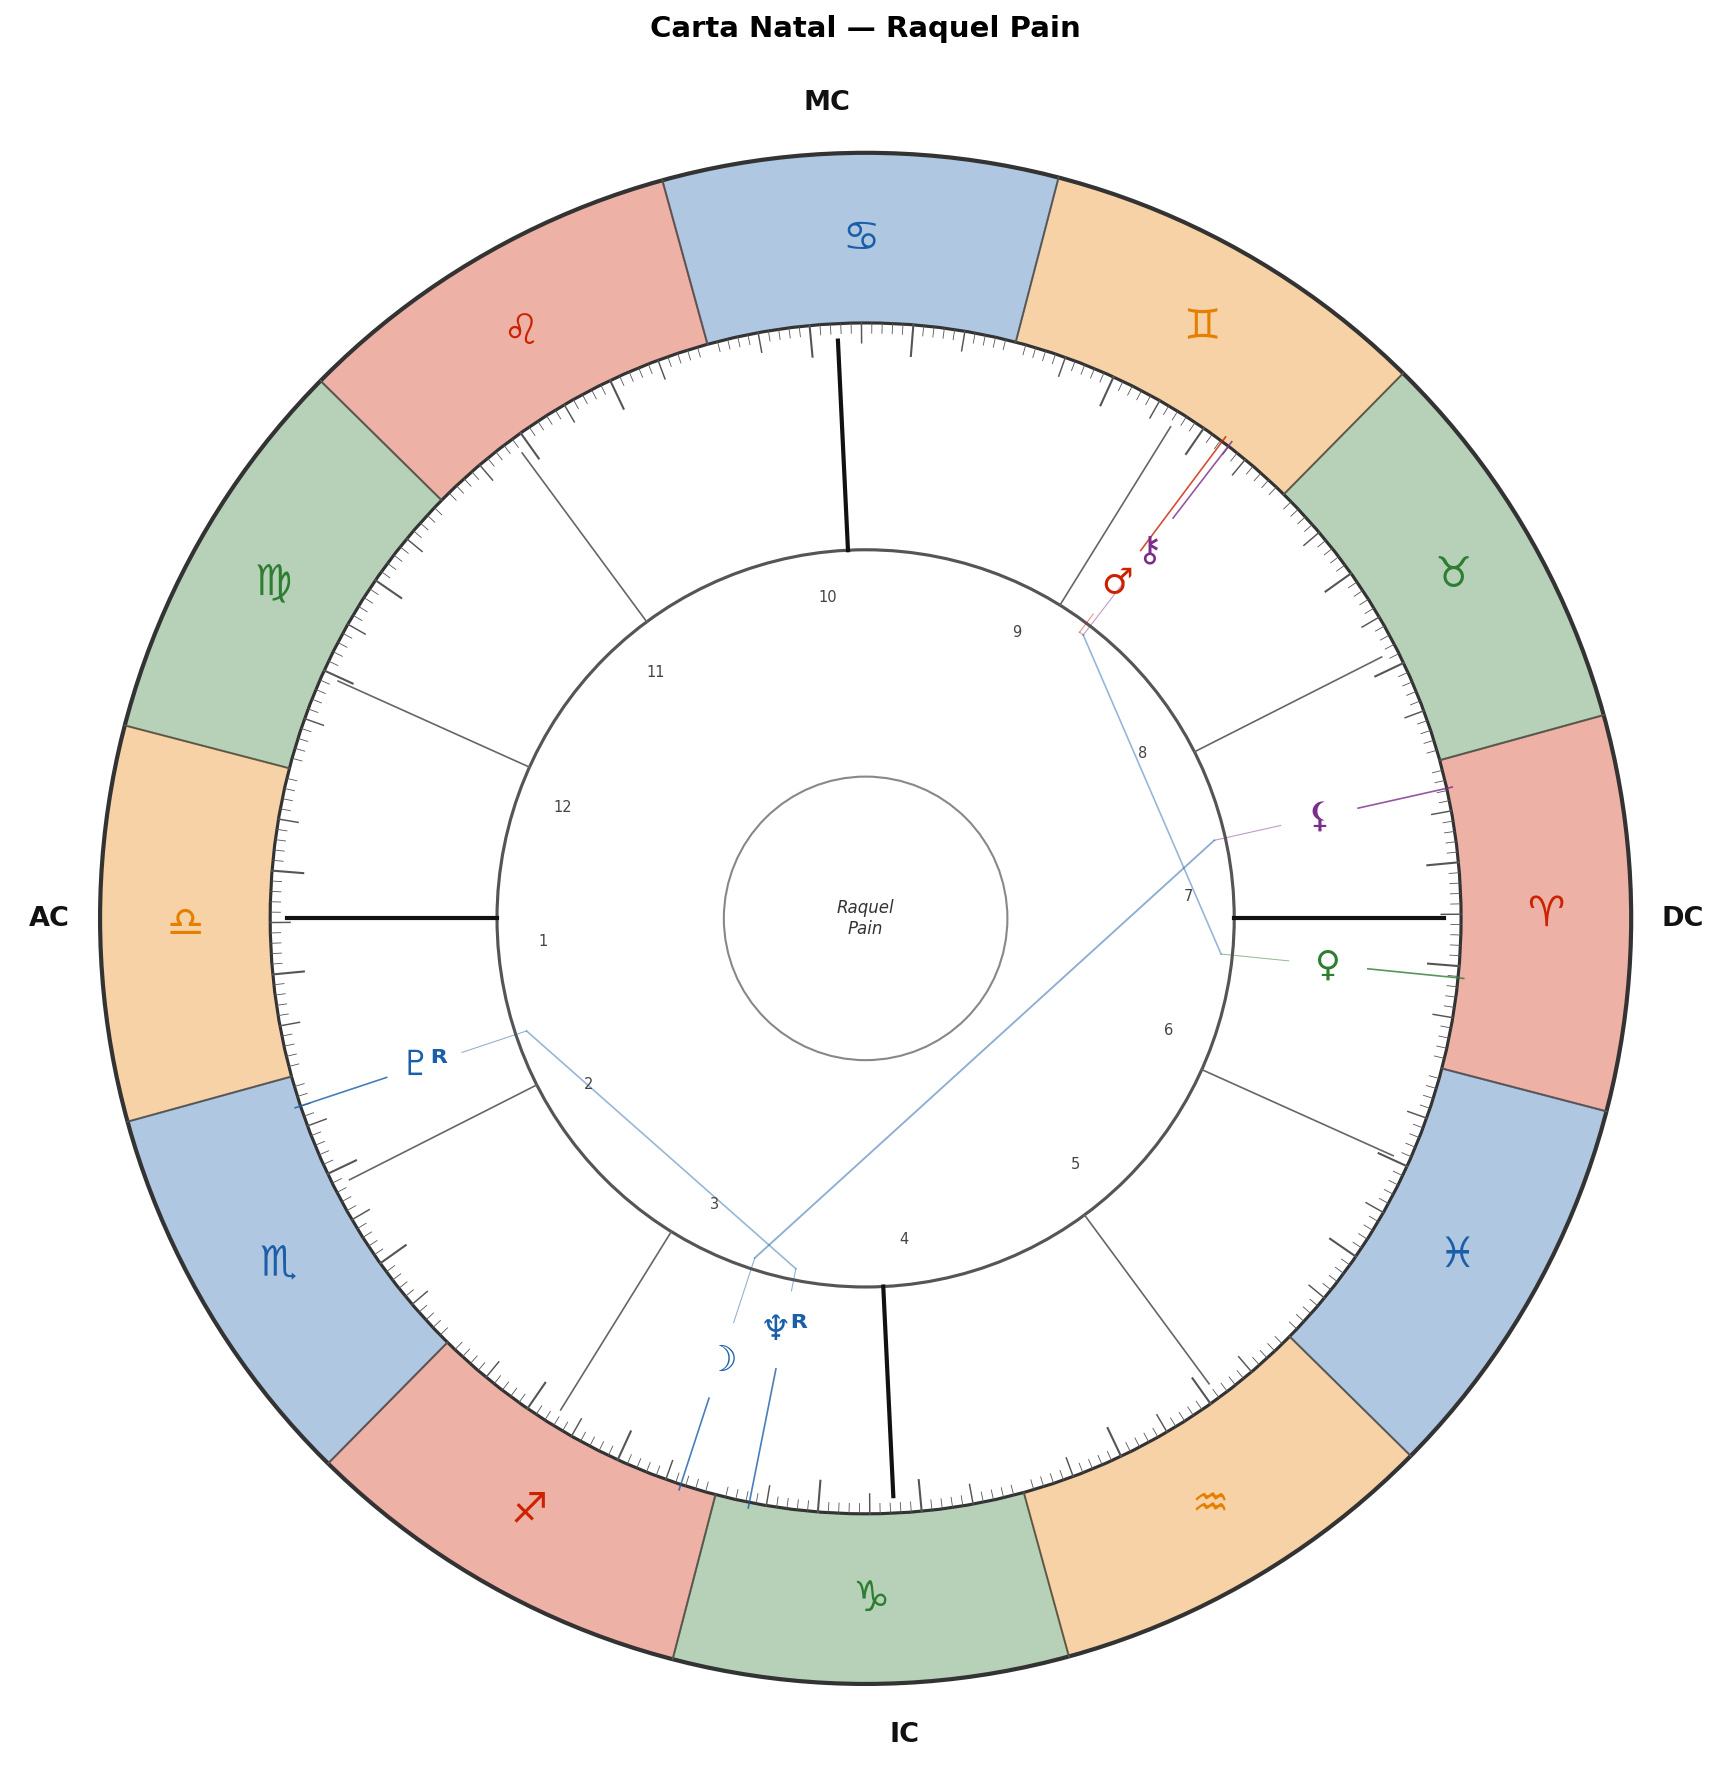
\includegraphics[width=0.72\textwidth]{Raquel_Pain_rueda.png}
\end{center}

\vspace{0.8cm}
\Needspace{5\baselineskip}


% ── Interpretación ───────────────────────────────────────────────────────────

\section{Interpretación — Arquitectura Interna}

\begin{center}
{\small\itshape
No se trata de definir quién eres.\\
Se trata de observar cómo tiendes a crecer, estructurarte\\
y sostener tu relación con el mundo.
}
\end{center}

\vspace{0.8cm}
\Needspace{5\baselineskip}

% ── 1. Estructura general ────────────────────────────────────────────────────

\subsection{1. Estructura general}

Júpiter está en Acuario, Casa 4: muestra cómo tiendes a crecer, abrir posibilidades y ampliar tu relación con el mundo.
Saturno está en Escorpio, Casa 2: muestra cómo tiendes a estructurarte, sostener límites y construir estabilidad.

Expansión (Acuario, Aire) y estructura (Escorpio, Agua) operan en elementos que crean tensión. Puede haber momentos en los que crecer y sostenerte requieran movimientos internos diferentes, por lo que la integración necesita más atención consciente.

Aspectos relevantes: Júpiter–Sol en cuadratura (orbe 1.31°), Júpiter–Mercurio en sextil (orbe 5.47°), Júpiter–Marte en trígono (orbe 7.91°), Júpiter–Urano en sextil (orbe 1.42°), Saturno–Sol en oposición (orbe 8.39°).

\vspace{0.8cm}
\Needspace{5\baselineskip}

% ── 2. Júpiter ───────────────────────────────────────────────────────────────

\subsection{2. Júpiter — Expansión y crecimiento}

\subsubsection*{
Júpiter en Acuario
— Casa 4
}

Tiendes a crecer a través de la innovación, la apertura mental y la posibilidad de aportar algo diferente. La expansión aparece cuando puedes cuestionar estructuras existentes y participar en algo más amplio que lo estrictamente personal. Necesitas libertad mental y espacio para pensar distinto.

En situaciones de desbordamiento: puedes perder contacto con lo concreto y quedar atrapada en ideas que nunca llegan a materializarse. La distancia emocional o la abstracción excesiva dificultan la integración real. En momentos de estancamiento: si no encuentras un contexto donde sentir que tu visión tiene sentido, la motivación disminuye mucho. La falta de conexión con algo colectivo o significativo puede bloquear la dirección de crecimiento.

Tiendes a crecer desde la base interior, la intimidad y la sensación de pertenencia. La expansión aparece cuando existe suficiente seguridad emocional y un espacio propio desde el que sostenerte. Necesitas raíces sólidas antes de extenderte hacia fuera.

Júpiter cuadratura Sol: la necesidad de crecer y la dirección que intentas sostener generan tensión. Puedes querer expandirte más allá de lo que realmente puedes integrar o sentir que la dirección actual resulta demasiado estrecha para lo que necesitas desarrollar.

La dificultad suele aparecer al medir límites, ritmos y capacidad real de sostén.

\vspace{0.8cm}
\Needspace{5\baselineskip}

% ── 3. Saturno ───────────────────────────────────────────────────────────────

\subsection{3. Saturno — Estructura y sostén}

\subsubsection*{
Saturno en Escorpio
— Casa 2 (Retrógrado)
}

Tiendes a estructurarte a través del control de lo importante y la profundidad emocional. Necesitas sentir que puedes confiar en lo que entra dentro de tu vida y comprender lo que ocurre bajo la superficie. La estructura aparece delimitando cuidadosamente qué merece acceso a tu espacio interno.

El límite aparece en la dificultad para confiar plenamente o soltar el control. No todo puede verificarse antes de abrirse.

Cuando la estructura deja de sostenerse: el control reemplaza la capacidad de organizar y contener. La vigilancia constante termina consumiendo mucha energía y dificultando la flexibilidad.

Tiendes a estructurarte a través de los recursos, la estabilidad y la gestión de lo que tiene valor para ti. La seguridad suele construirse lentamente, mediante constancia y acumulación progresiva. Necesitas sentir que existe una base concreta sobre la que apoyarte.

El límite aparece cuando intentas sostener más de lo que tus recursos reales permiten. La estabilidad depende de la capacidad de administrar energía, tiempo y recursos de forma sostenible.

Saturno está retrógrado. La construcción de estructura suele desarrollarse de forma más interna y menos visible desde fuera al principio. Puedes necesitar tiempo antes de mostrar externamente algo que por dentro todavía estás consolidando.

Saturno oposición Sol: dirección y estructura tienden a tirar en sentidos diferentes. Cuando avanzas hacia lo que quieres desarrollar, puedes sentir peso, límite o resistencia. Cuando priorizas estabilidad o control, la dirección vital pierde fuerza.

Necesitas aprender a construir sin apagar completamente el impulso vital.

\vspace{0.8cm}
\Needspace{5\baselineskip}

% ── 4. Integración ───────────────────────────────────────────────────────────

\subsection{4. Integración — Crecimiento y estructura}

Júpiter en Acuario (Aire) y Saturno en Escorpio (Agua) no forman aspecto directo, pero operan en elementos que crean tensión. Esto puede hacer que crecer y sostenerte requieran movimientos internos diferentes. La expansión y la estructura no se alimentan de forma automática; necesitas integrarlas de manera consciente para no abrir posibilidades sin sostén ni construir estructuras sin crecimiento real.

Cuando Júpiter domina: puedes multiplicar perspectivas, ideas y conexiones sin que ninguna llegue a profundizar o tomar forma. La estructura de Saturno en Escorpio no compensa con suficiente rapidez y lo que ganas en amplitud empieza a perder forma.

Cuando Saturno domina: la contención puede suprimir lo que necesita circular, y lo no expresado se acumula. La expansión de Júpiter en Acuario no encuentra espacio para activarse y puedes mantener lo que ya existe sin crecer hacia lo que sería posible.

Bajo presión suele aparecer una secuencia bastante reconocible. Primero, Saturno en Escorpio empieza a ceder: los límites emocionales se diluyen y deja de existir suficiente contención. Después, Júpiter en Acuario ocupa ese espacio: multiplicas conexiones, ideas o perspectivas sin que lleguen a integrarse de forma coherente. Desde ahí puedes intentar recuperar estabilidad rápidamente, pero lo que construyes en ese estado suele ser más rígido, reactivo o agotador de sostener. Si el patrón no se reconoce a tiempo, el ciclo tiende a repetirse.

\vspace{0.8cm}
\Needspace{5\baselineskip}

% ── 5. Orientación práctica ──────────────────────────────────────────────────

\subsection{5. Orientación práctica}

\subsubsection*{Desde dónde empezar}

El punto de entrada más accesible suele estar en la expansión (Acuario, Casa 4). De las dos funciones, esta requiere menos resistencia para activarse. La forma más natural de empezar es poner en palabras, compartir o mover lo que ya está disponible. Cuando todo parece bloqueado, comenzar por aquí suele facilitar que la otra función también pueda ponerse en marcha.

\subsubsection*{Qué sostener}

Lo más importante de sostener aparece en Saturno (Escorpio, Casa 2). Bajo presión puedes abrir posibilidades o reaccionar antes de mantener forma estable. Conviene cuidar especialmente mantener límites emocionales suficientes para no saturarte. Muchas veces la primera señal de desgaste aparece cuando sigues haciendo cosas, pero ya no existe suficiente estructura para sostenerlas bien.

\subsubsection*{Qué evitar}

Conviene evitar que la función más activa en cada momento desplace completamente a la otra. Con Júpiter en Acuario (Aire) y Saturno en Escorpio (Agua), crecimiento y estructura no se activan automáticamente juntos. Necesitas reconocer conscientemente cuándo hace falta abrir más espacio y cuándo hace falta construir más sostén.

\subsubsection*{Si no se integra}

Cuando crecimiento y estructura dejan de colaborar, puede aparecer expansión sin suficiente sostén o estabilidad sin movimiento real. En ambos casos se pierde parte de lo que realmente podría desarrollarse si ambas funciones trabajaran en la misma dirección.

\subsubsection*{Señal temprana}

La primera señal suele aparecer en Saturno (Escorpio): los límites emocionales dejan de contener suficientemente. Cuando eso ocurre, Júpiter (Acuario) tiende a ocupar rápidamente el espacio disponible y la expansión puede acelerarse más de lo que realmente puedes sostener. Detectar la señal temprano suele evitar entrar en ciclos más agotadores.

\vfill

\begin{center}
{\small\itshape\color{grisai}
La astrología se utiliza aquí como herramienta simbólica de observación\\
y no como una definición cerrada de la persona.
}
\end{center}

\end{document}
